\documentclass[landscape]{baposter}

\usepackage[vlined]{algorithm2e}
\usepackage{times}
\usepackage{calc}
\usepackage{url}
\usepackage{graphicx}
\usepackage{amsmath}
\usepackage{amssymb}
\usepackage{relsize} 
\usepackage{multirow}
\usepackage{booktabs}
\usepackage{setspace}
\usepackage{graphicx}
\usepackage{multicol}
\usepackage[T1]{fontenc}
\usepackage{ae}
%\usepackage{xcolor}
\usepackage{color}
\graphicspath{{images/}}

\definecolor{SUblue}{RGB}{0,51,102}
%\definecolor{SUblue}{RGB}{15,77,146}
\definecolor{scrpink}{RGB}{167, 87, 168}
\setlength{\columnsep}{0.7em}
\setlength{\columnseprule}{0mm}
\begin{document}
\begin{poster}{
 % Show grid to help with alignment
 grid=no,
 % Column spacing
 colspacing=0.7em,
 % Color style
% headerColorOne=cyan!20!white!90!black,
% borderColor=cyan!30!white!90!black,
%headerColorOne=SUblue!90!white!90!black,
 headerColorOne=SUblue,
 borderColor=orange!90!white!90!black,
 % Format of textbox
 textborder=faded,
 % Format of text header
 headerborder=open,
 headershape=roundedright,
 background=none,
 bgColorOne=cyan!10!white,
 headerheight=0.12\textheight}
 % Eye Catcher
 {
       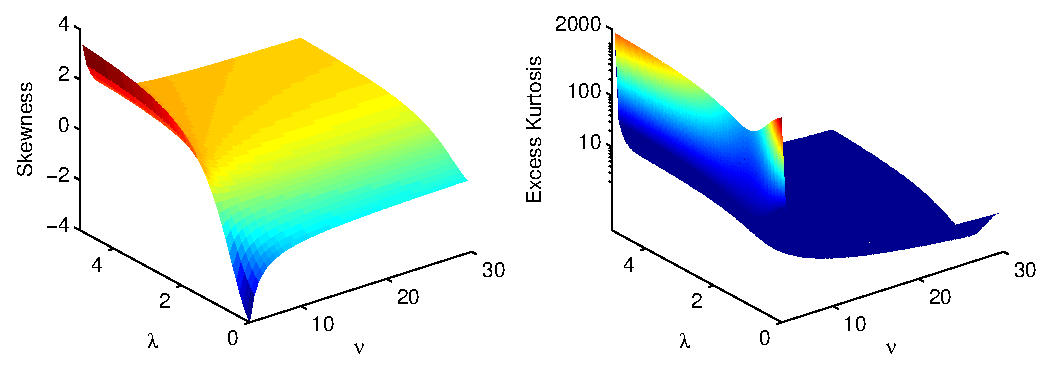
\includegraphics[height=0.12\textheight]{skewness}
      % 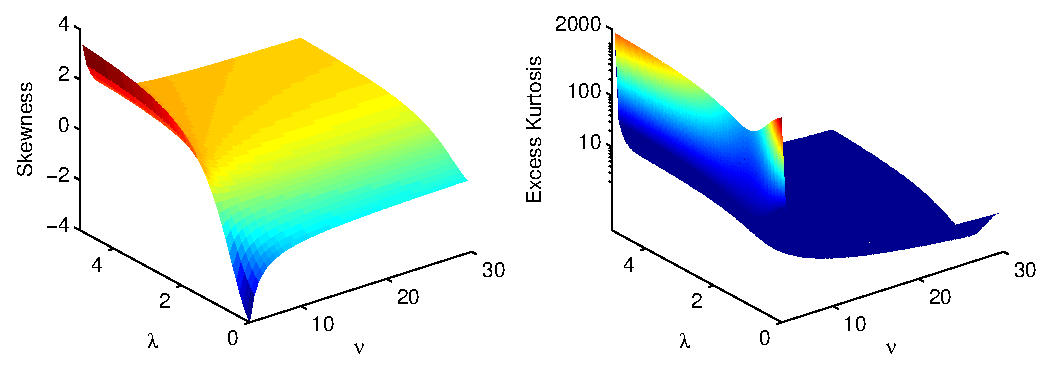
\includegraphics[width=0.08\linewidth]{skewness}
%      \includegraphics[width=0.08\linewidth]{track_frame_04999_06}
 }
 % Title
 {\Huge Smooth Mixtures of
    Asymmetric Student \emph{t} Densities \newline}
 % Authors
{{\sc Feng Li, Department of Statistics, Stockholm University, Sweden}\\[0.5em]
\scalebox{0.85}{\sc joint with Mattias Villani and Robert Kohn}}
 % University logo 
 {
  \begin{tabular}{r}
    
\includegraphics[height=0.12\textheight]{sulogo}\\
 %   \raisebox{0em}[0em][0em]{
\includegraphics[height=0.05\textheight]{statlogo}}
  \end{tabular}
 }

 \headerbox{\color{white}{Contributions}}{name=contribution,column=0,row=0,span=2}{
  A general model is proposed for flexibly estimating the density of a continuous response
  variable conditional on a possibly high-dimensional set of covariates. The model is a
  finite mixture of asymmetric student-\emph{t} densities with covariate-dependent mixture
  weights. The four parameters of the components, the mean, degrees of freedom, scale and
  skewness, are all modeled as functions of the covariates.
  }

  \headerbox{\color{white}{Asymmetric Student \emph{t}}}{name=split-t,column=0,below=contribution}{
    The split-\emph{t} density is
\[
f\left( {y;\mu ,\phi ,\lambda ,\nu } \right) = \begin{cases} 
c \cdot \kappa \left( {y;\mu ,\phi ,\nu} \right); &\text{if } y \leq \mu, \\
 c \cdot \kappa \left( {y;\mu ,\lambda \phi ,\nu} \right); &\text{if } y > \mu,
\end{cases}
\]
where $ \kappa \left( {y;\mu ,\phi ,\nu} \right) $ is the kernel of student \emph{t} density and $c$ is the normalization constant.
%\begin{figure}
\begin{center}
  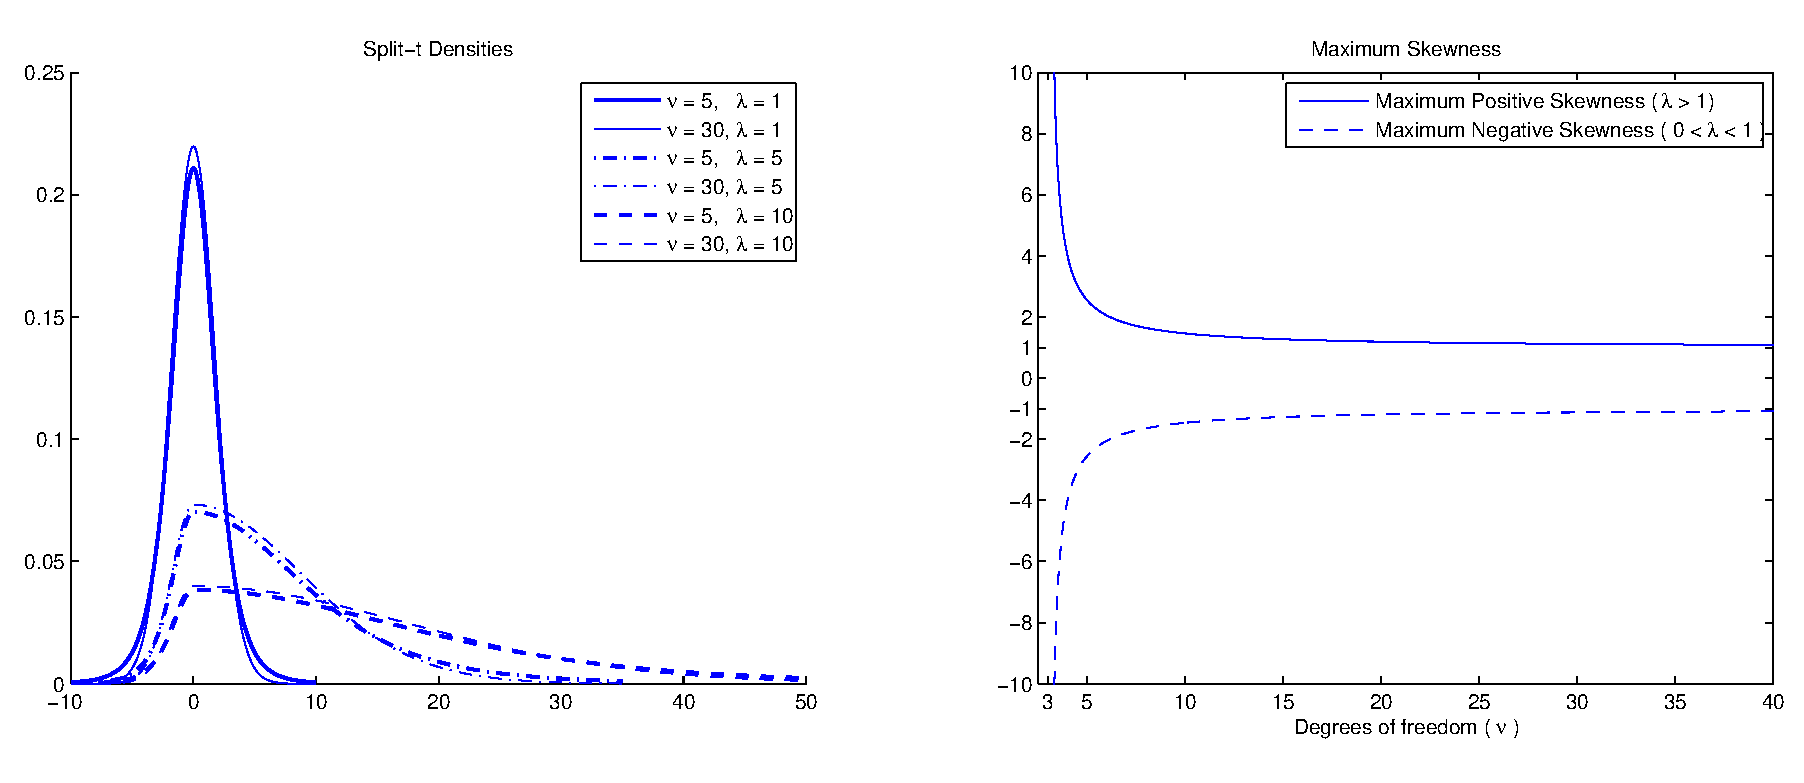
\includegraphics[width=0.80\textwidth]{Density_Skewness}   
\end{center}
% \begin{center}
% 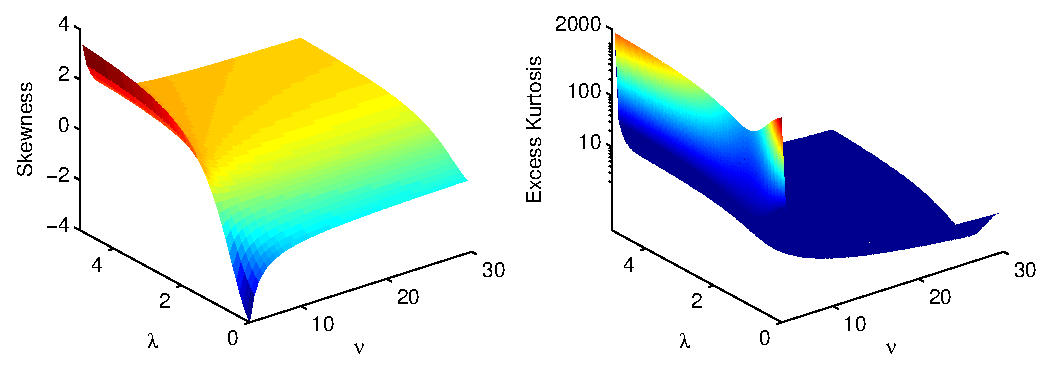
\includegraphics[width=0.80\textwidth]{skewness}
% \end{center}
% \end{figure}
\color{orange}{\emph{\textbf{Basic Properties:}}}\vspace{0.2cm}
\begin{spacing}{0.7}
{\scriptsize \color{blue}{
\indent \hspace{0.7cm} 1. $\lambda<1$, skewed to the left; $\lambda>1$, skewed to the
right;\\
\indent \hspace{0.7cm} 2. $\lambda=1$,  reduces to symmetric student-\emph{t} distribution;\\
\indent \hspace{0.7cm} 3. $\nu\rightarrow\infty$, reduces to the two-piece normal
distribution;\\
\indent \hspace{0.7cm} 4.  $\lambda=1$ and $\nu\rightarrow\infty$, reduces to normal distribution.
}}
\end{spacing}

}
 %%%%%%%%%%%%%%%%%%%%%%%%%%%%%%%%%%%%%%%%%%%%%%%%%%%%%%%%%%%%%%%%%%%%%%%%%%%%%%
   \headerbox{\color{white}{Mixture of Split-\emph{t}}}{name=data,column=0,above=bottom,below=split-t}{
 %%%%%%%%%%%%%%%%%%%%%%%%%%%%%%%%%%%%%%%%%%%%%%%%%%%%%%%%%%%%%%%%%%%%%%%%%%%%%%
Given $x$, a finite mixture distribution $p(y|x)$ is 
  \[
  \sum\nolimits_{k = 1}^K {\omega _k f_k \left( {y_i |\theta _k } \right),~i = 1,...,n.} 
  \]
A smooth mixture model is a finite mixture density with weights that are smooth function
of the covariates, e.g 
\[
\omega _k \left( x \right) = \frac{{\exp \left( {x'\gamma _k } \right)}}
{{\sum\nolimits_{r = 1}^K {\exp \left( {x'\gamma _r } \right)} }}
\]
In a smooth mixture of split-\emph{t} densities, the four components $\mu,\phi,\lambda$
and $\nu$ in each mixture components are connected to covariates as, e.g.,
\[
\begin{array}{*{20}c}
   {~~~\mu  = \beta _{\mu _0 }  + x_t '\beta _\mu  ,} & {\ln \phi  = \beta _{\phi _0 }  + x_t '\beta _\phi  ,}  \\
   {\ln \nu  = \beta _{\nu _0 }  + x_t '\beta _\nu  ,} & {\ln \lambda  = \beta _{\lambda _0 }  + x_t '\beta _\lambda  .}  \\
 \end{array} 
\]
{\emph{\color{orange}\textbf{Features are common}}} if only the intercepts are allowed to
be different across components. This often an empirically relevant, simplification of the model.
}
 %%%%%%%%%%%%%%%%%%%%%%%%%%%%%%%%%%%%%%%%%%%%%%%%%%%%%%%%%%%%%%%%%%%%%%%%%%%%%%%
   \headerbox{\color{white}{Key Features}}{name=features,column=1,below=contribution}{
 %%%%%%%%%%%%%%%%%%%%%%%%%%%%%%%%%%%%%%%%%%%%%%%%%%%%%%%%%%%%%%%%%%%%%%%%%%%%%%%
     \begin{enumerate}
     \item {\color{orange}\emph{\textbf{Complex-but-few}}} approach -- Enough flexibility is used within the mixture
       components so that the number of components can be kept to a minimum.
     \item {\color{orange}\emph{ \textbf{Bayesian variable selection}}} are used in all five sets of covariates in mean, scale,
       skewness and kurtosis parameters and gating function to automatically determine
       important variables.
\begin{center}
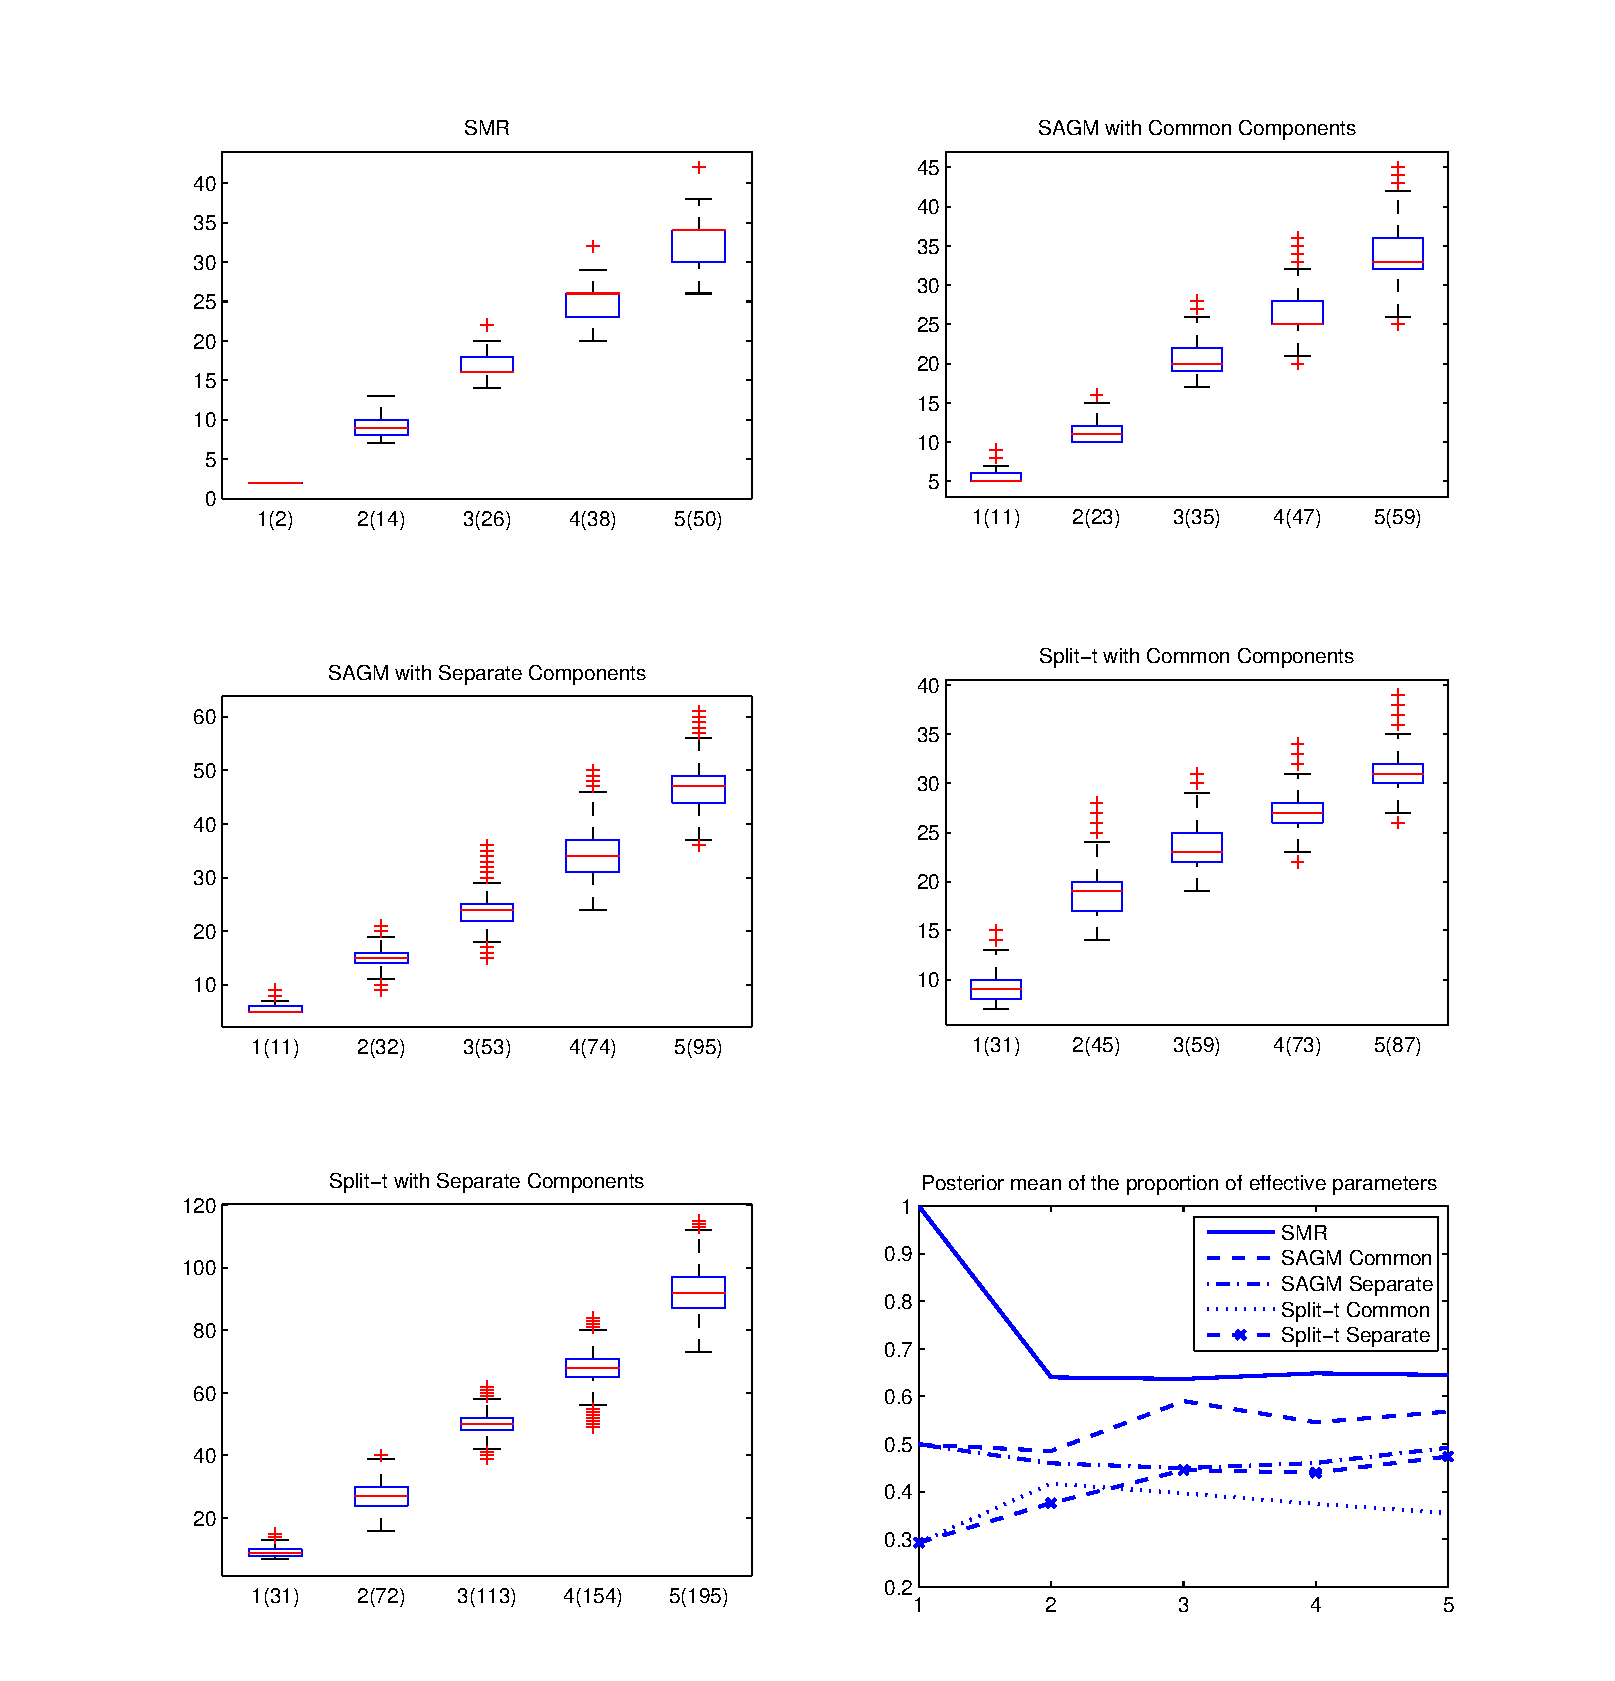
\includegraphics[width=0.8\textwidth]{ParametersSizeBoxPlot}
\end{center}
\begin{spacing}{0.7}
{\scriptsize \color{blue}{The figure displays the posterior distributions of the number of included
  parameters in the S\&P 500 data. On first five subplots, the horizontal 
axis measures the number of components (potential number of parameters in parentheses) and the vertical
axis is the total number of effective parameters after variable selection. The
right-bottom subplot is the posterior mean of the proportion of effective parameters in
each model.}}
\end{spacing}

     \item {\color{orange}\emph{\textbf{Finite-step Newton's method}}} within variable
             selection is used to sample the parameters which can greatly speed up the algorithm.  
     \item {\color{orange}\emph{\textbf{Five-fold cross-validation}}} of the log predictive
       density score(LPDS) is used in model comparison.
     \end{enumerate}


}
 %%%%%%%%%%%%%%%%%%%%%%%%%%%%%%%%%%%%%%%%%%%%%%%%%%%%%%%%%%%%%%%%%%%%%%%%%%%%%%
   \headerbox{\color{white}{Applications}}{name=name-2,column=2,row=0,span=2}{
 %%%%%%%%%%%%%%%%%%%%%%%%%%%%%%%%%%%%%%%%%%%%%%%%%%%%%%%%%%%%%%%%%%%%%%%%%%%%%%
Financial data, such as stock market returns, are typically heavy tailed and subject to volatility
clustering. The model is applied to analyse the distribution of daily
stock market returns conditional on nine covariates and outperforms widely used GARCH models
and other recently proposed mixture models in an out-of-sample evaluation of returns during the
recent financial crisis.
   }


 %%%%%%%%%%%%%%%%%%%%%%%%%%%%%%%%%%%%%%%%%%%%%%%%%%%%%%%%%%%%%%%%%%%%%%%%%%%%%%

\headerbox{\color{white}{Daily S\&P 500 Returns}}{name=data,column=2,span=1,below=name-2,above=bottom}{
 %%%%%%%%%%%%%%%%%%%%%%%%%%%%%%%%%%%%%%%%%%%%%%%%%%%%%%%%%%%%%%%%%%%%%%%%%%%%%%
\begin{center}
    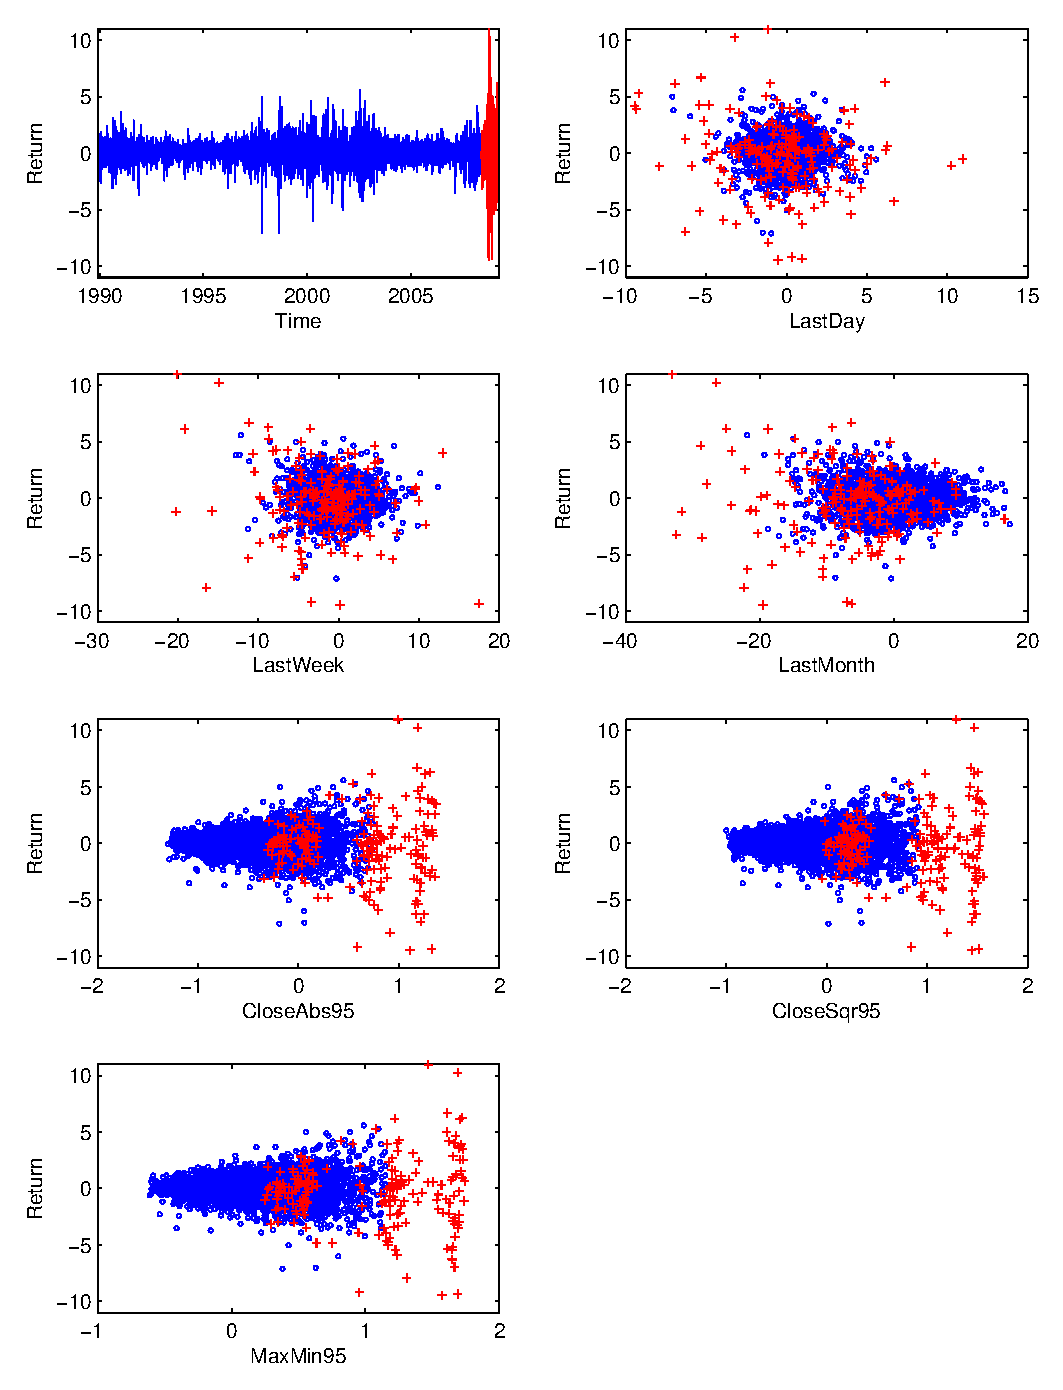
\includegraphics[width=0.46\textwidth]{SP500Data} 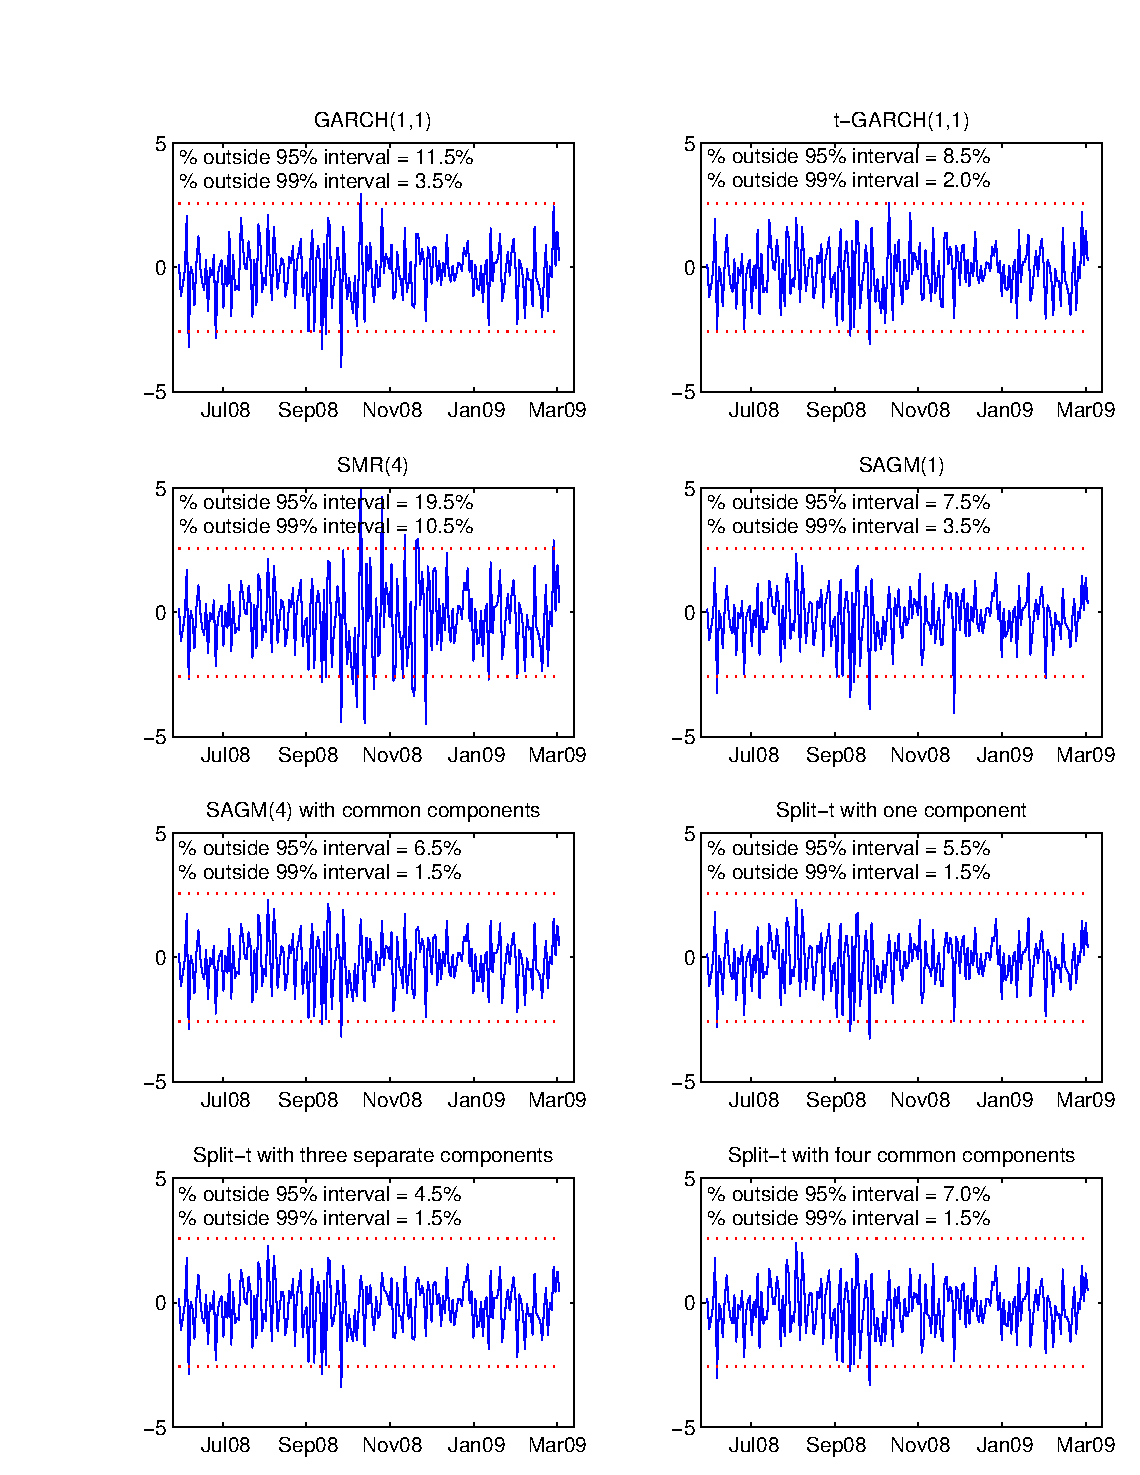
\includegraphics[width=0.51\textwidth]{normResidPlot} 
\end{center}
We use normalized residuals to assess the quality of the predictive densities. The
SMR (\emph{simple-and-many} approach) with largest LPDS produces much to large residuals during the most 
volatile period, and so does the GARCH(1,1) and \emph{t}-GARCH(1, 1). The
one-component split-\emph{t} model is doing remarkably well during this very difficult
time period. 
\begin{center} 
\scalebox{0.54}{
\begin{tabular}{lccccccc}
% &  &  &  &  &  &  & \tabularnewline
\hline
\hline 
 &  &  &  &  &  &  & \tabularnewline
Model & $K=1$ & $K=2$ & $K=3$ & $K=4$ & $K=5$   & Max n.s.e.\tabularnewline
\hline
 &  &  &  &  &   & \tabularnewline
SMR & ${\color{red}\mathbf{-1044.78}}$ & $-638.89$ & $-505.74$ & $-487.11$ & $-489.19$   & $0.98\,(3)$\tabularnewline
+ Skew & $-540.91$ & $-525.07$ & $-513.85$ & $-506.68$ & $-506.13$  & $0.82\,(2)$\tabularnewline
+ DF & $-544.00$ & $-518.71$ & $-498.93$ & $-500.14$ & $-494.29$   & $0.89\,(1)$\tabularnewline
+ Skew + DF & $-530.86$ & $-504.63$ & $-498.03$ & $-498.83$ & ${\color{red}\mathbf{-496.87}}$   & $0.88\,(5)$\tabularnewline
 &  &  &  &  &    & \tabularnewline
SAGM Common & $-477.73$ & $-473.10$ & $-473.12$ & $-470.30$ & $-472.86$  & $0.26\,(2)$\tabularnewline
+ Skew & $-474.18$ & $-467.29$ & $-468.75$ & $-467.93$ & $-467.22$   & $0.35\,(4)$\tabularnewline
+ DF & $-474.74$ & $-472.92$ & $-470.51$ & $-469.40$ & $-468.87$   & $0.34\,(4)$\tabularnewline
+ Skew + DF & $ {\color{blue}\mathbf{-472.37}}$ & $-468.92$ & $-469.30$ & $-466.21$ & {\color{blue}\textbf{$\mathbf{-465.86}$}}   & $0.53\,(4)$\tabularnewline
 &  &  &  &  &   & \tabularnewline
SAGM Separate &  & $-469.21$ & $-469.50$ & $-470.53$ & $-471.02$   & $0.49\,(3)$\tabularnewline
+ Skew &  & $-468.48$ & $-466.93$ & $-467.48$ & $-468.02$   & $0.58\,(4)$\tabularnewline
+ DF &  & $-469.08$ & $-469.24$ &  {\color{blue}\textbf{$\mathbf{-462.03}$}} & $-467.78$   & $0.72\,(5)$\tabularnewline
+ Skew + DF &  & $ {\color{blue}\mathbf{-466.84}}$ & $ {\color{blue}\mathbf{-462.56}}$ & $-462.47$ & $-474.58$   & $0.74\,(5)$\tabularnewline
 &  &  &  &  &    & \tabularnewline
GARCH(1,1) & $-479.03$ &  &  &  &   & \tabularnewline
$t$-GARCH(1,1) & $-477.39$ &  &  &  &   & \tabularnewline
&  &  &  &  &   & \tabularnewline
\hline
\hline
 &  &  &  &  &   & \tabularnewline
\end{tabular}  
}
\end{center} 
LPDS shows that the SMR model does poorly, even with a large number of
components, and is outperformed by the GARCH(1, 1) and \emph{t}-GARCH(1, 1) models.
The split-t with covariate dependent scale,
skewness and degrees of freedom is the best one-component model.
%}
}
 %%%%%%%%%%%%%%%%%%%%%%%%%%%%%%%%%%%%%%%%%%%%%%%%%%%%%%%%%%%%%%%%%%%%%%%%%%%%%%
   \headerbox{\color{white}{Posterior Study}}{name=moments, row = 0,column=3, below=name-2, span
     = 1}{
 %%%%%%%%%%%%%%%%%%%%%%%%%%%%%%%%%%%%%%%%%%%%%%%%%%%%%%%%%%%%%%%%%%%%%%%%%%%%%%
\begin{center}
    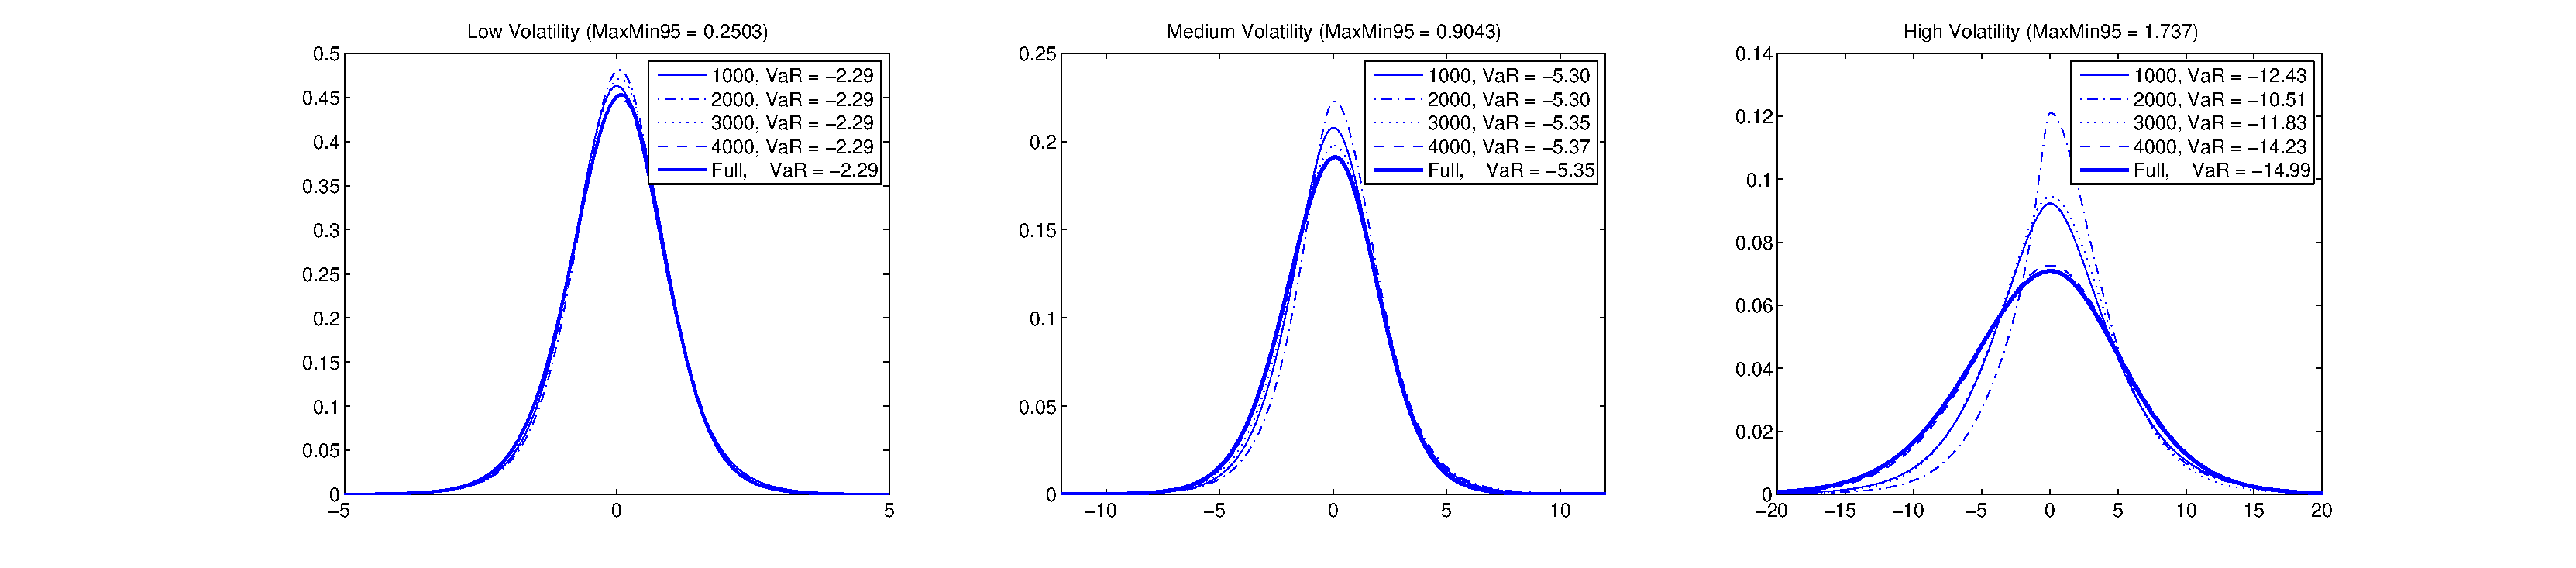
\includegraphics[width=\textwidth]{Volatility23}
\end{center}
We estimate one-component split-\emph{t} model using first 1000, 2000, 3000, 4000 trading
days and the full 
sample. Then we obtain conditional predictive densities for three sets of covariates
low, medium and high volatility. It is shown that the predictive densities is 
stable even with very high volatility data.
\begin{center}
    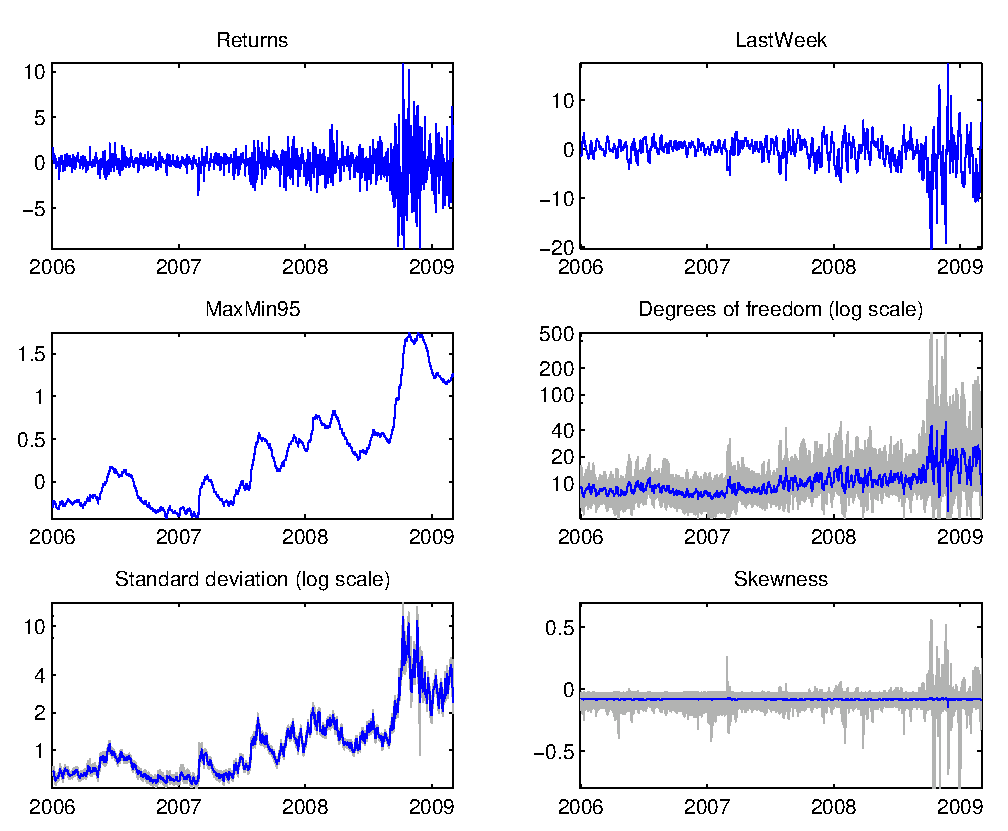
\includegraphics[width=0.80\textwidth]{MomentPlotSP500} 
\end{center}
The median of the degrees of freedom actually increased during the most volatile part of the financial
crisis (but at the same time the scale parameter rose dramatically to bring about a very large boost
in standard deviation of returns), but, during some spells, the posterior distribution of $\nu$ also has
a long left tail with substantial probability mass on very small values of $\nu$.
   }

   \headerbox{\color{white}{Footnotes}}{name=note, column=3, above=bottom,below=moments}{
\begin{spacing}{0.7}
{\tiny Li (feng.li@stat.su.se) is a Ph.D student at Stockholm 
  University. Villani (mattias.villani@gmail.com) is a researcher at Sveriges Riksbank and
  senior lecturer at Stockholm 
  University. Kohn (r.kohn@unsw.edu.au) is Scientia Professor at the Australian School of
  Business, University of New South Wales. Kohn was partially supported by ARC Grant DP0667069. This paper is forthcoming in \emph{Journal of Statistical Planning and Inference,} {\color{blue}doi:10.1016/j.jspi.2010.04.031}.} 
\end{spacing}
}
\end{poster}%
%
\end{document}